
%(BEGIN_QUESTION)
% Copyright 2006, Tony R. Kuphaldt, released under the Creative Commons Attribution License (v 1.0)
% This means you may do almost anything with this work of mine, so long as you give me proper credit

Shown here is a very simple {\it pressure transmitter}, a device that measures a fluid pressure and converts that measurement into an electrical signal:

$$\includegraphics[width=15.5cm]{i00083x01.eps}$$

Suppose the potentiometer wiper will be at its full-down position with no pressure applied to the diaphragm, and will be at its full-up position with 15 PSI (15 pounds per square inch) of pressure applied to the diaphragm.  Based on this information, and what you see in the schematic diagram, answer the following questions:

\begin{itemize}
\item{} Lower Range Value (LRV) of input, in units of PSI:
\item{} Upper Range Value (URV) of input, in units of PSI:
\item{} Input span, in units of PSI:
\vskip 5pt
\item{} Lower Range Value (LRV) of output, in units of volts:
\item{} Upper Range Value (URV) of output, in units of volts:
\item{} Output span, in units of volts:
\end{itemize}

\goodbreak
Now, suppose we make a modification to the electrical circuit portion of the pressure transmitter.  Assume the diaphragm still responds to pressure and moves the potentiometer wiper the same way it did before.  Answer the same questions again:

$$\includegraphics[width=15.5cm]{i00083x02.eps}$$

\begin{itemize}
\item{} Lower Range Value (LRV) of input, in units of PSI:
\item{} Upper Range Value (URV) of input, in units of PSI:
\item{} Input span, in units of PSI:
\vskip 5pt
\item{} Lower Range Value (LRV) of output, in units of volts:
\item{} Upper Range Value (URV) of output, in units of volts:
\item{} Output span, in units of volts:
\end{itemize}

The latter design outputs what is commonly called a {\it live-zero} signal, whereas the first transmitter outputs a {\it dead-zero} signal.  Live-zero signals are much preferred in industrial instrumentation, because they more readily betray wiring failures than dead-zero signals.

\vskip 10pt

Explain how you answered all the questions, and also show currents and voltage drops in both circuits (complete with arrows showing directions of current).  Then, elaborate on why you think live-zero signals are preferable to dead-zero signals.

\underbar{file i00083}
%(END_QUESTION)





%(BEGIN_ANSWER)

\noindent
{\bf First transmitter design:}

Input range: 0 to 15 PSI

Output range: 0 to 10 volts DC

\vskip 10pt

\noindent
{\bf Last transmitter design:}

Input range: 0 to 15 PSI

Output range: 1 to 5 volts DC

\vskip 10pt

Follow-up question: show the current in both circuits using both conventional flow notation and electron flow notation.

%(END_ANSWER)





%(BEGIN_NOTES)

\noindent
{\bf First transmitter design:}

Input range: 0 to 15 PSI

Input span: 15 PSI

Output range: 0 to 10 volts DC

Output span: 10 volts DC

\vskip 10pt

\noindent
{\bf Last transmitter design:}

Input range: 0 to 15 PSI

Input span: 15 PSI

Output range: 1 to 5 volts DC

Output span: 4 volts DC (calculation: 5 volts $-$ 1 volt)

\vskip 10pt

$$\includegraphics[width=15.5cm]{i00083x03.eps}$$

$$\includegraphics[width=15.5cm]{i00083x04.eps}$$

In metallic conductors, electrons are the dominant carriers of electrical charge, and so electron flow is technically the ``correct'' way to represent the flow of electricity in a DC circuit.  However, conventional flow notation (where we assume that positively-charged particles move the other way) possesses some distinct advantages from a conceptual point of view.  First, it makes more sense when viewed from the perspective of a ``fluid analogy'' model of electricity.  For someone accustomed to thinking in terms of water flowing through pipes (current), and water pressure being analogous to electrical voltage, ``positive'' implies a region of high pressure while ``negative'' implies a region of low(er) pressure, so it makes sense to think of current flowing from the positive (high-pressure) side of a pump back around to the negative (low-pressure, or suction) side of a pump.

Secondly, conventional flow is used almost exclusively in science and engineering because the mathematical model of electromagnetism was originally constructed with this view in mind, when scientists honestly did not know better.  The ``right-hand rule'' of vector cross-products -- used when calculating forces and directions in electromagnetic systems -- only works when you imagine all electric currents as motions of positively-charged particles.  In keeping with this philosophy, all semiconductor components such as diodes and transistors show their symbol arrows pointing in the direction of conventional flow.  Students learning electron flow (the ``correct'' way of showing current in metal wires) must draw their currents going {\it against} the arrows inside diode and transistor symbols, which is a major source of confusion.

Truth be known, either way of visualizing electric current works just fine, so long as you are consistent in your notation.  It is very easy to get mixed up if you repeatedly switch from one notation to another.  The vast majority of my example diagrams are shown drawn in conventional flow notation.

\vskip 20pt \vbox{\hrule \hbox{\strut \vrule{} {\bf Virtual Troubleshooting} \vrule} \hrule}

This question is a good candidate for a ``Virtual Troubleshooting'' exercise.  Presenting the diagram to students, you first imagine in your own mind a particular fault in the system.  Then, you present one or more symptoms of that fault (something noticeable by an operator or other user of the system).  Students then propose various diagnostic tests to perform on this system to identify the nature and location of the fault, as though they were technicians trying to troubleshoot the problem.  Your job is to tell them what the result(s) would be for each of the proposed diagnostic tests, documenting those results where all the students can see.

During and after the exercise, it is good to ask students follow-up questions such as:

\begin{itemize}
\item{} What does the result of the last diagnostic test tell you about the fault?
\item{} Suppose the results of the last diagnostic test were different.  What then would that result tell you about the fault?
\item{} Is the last diagnostic test the best one we could do?
\item{} What would be the ideal order of tests, to diagnose the problem in as few steps as possible?
\end{itemize}

%INDEX% Basics, transmitter: input and output ranges
%INDEX% Basics, transmitter: live zero versus dead zero

%(END_NOTES)


